\question{Câu 2}

Tìm công thức liên hệ giữa $I_{L}$ và $V_{i}$ (Hình 2a) và giữa $I_{L}$ và $V_{1} - V_{2}$ (Hình 2b).

\begin{minipage}{.5\linewidth}
	\begin{figure}[H]
		\centering
		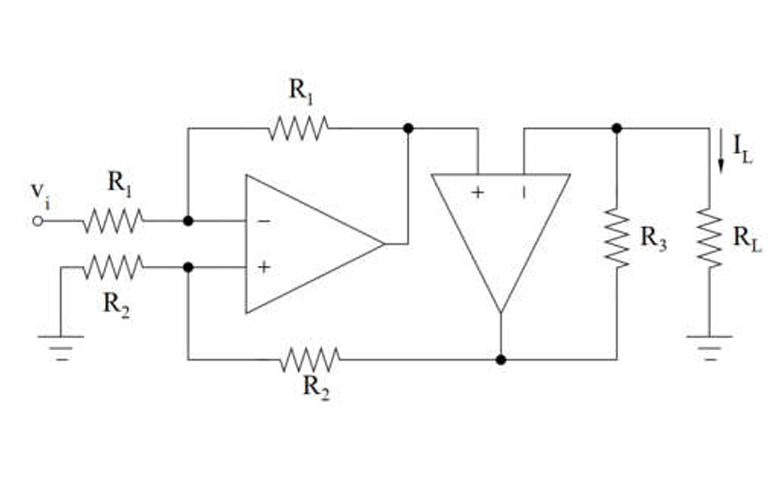
\includegraphics[width=\linewidth]{./my-chapters/my-images/Question2/debai_a.png}
		\caption*{Hình 2a.}
		\label{fig:Hinh2a_debai}
	\end{figure}
\end{minipage}
\begin{minipage}{.5\linewidth}
\begin{figure}[H]
	\centering
	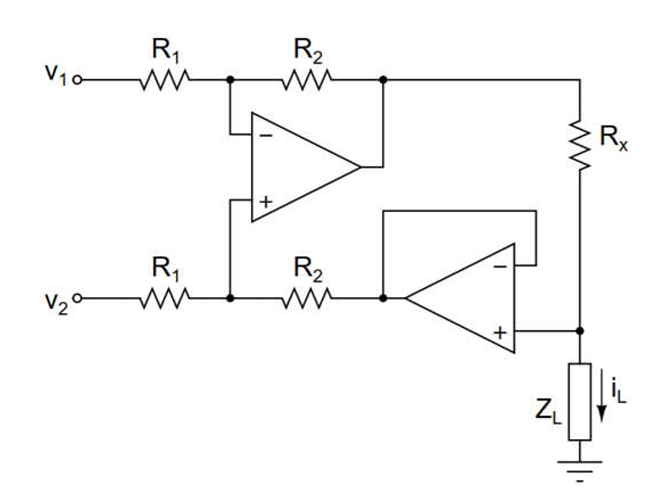
\includegraphics[width=\linewidth]{./my-chapters/my-images/Question2/debai_b.png}
	\caption*{Hình 2b.}
	\label{fig:Hinh2b_debai}
\end{figure}
\end{minipage}

\answer{a1}{Giả sử OPAMP ở hình 2a đang dùng là lý tưởng.}

\begin{figure}[H]
	\centering
	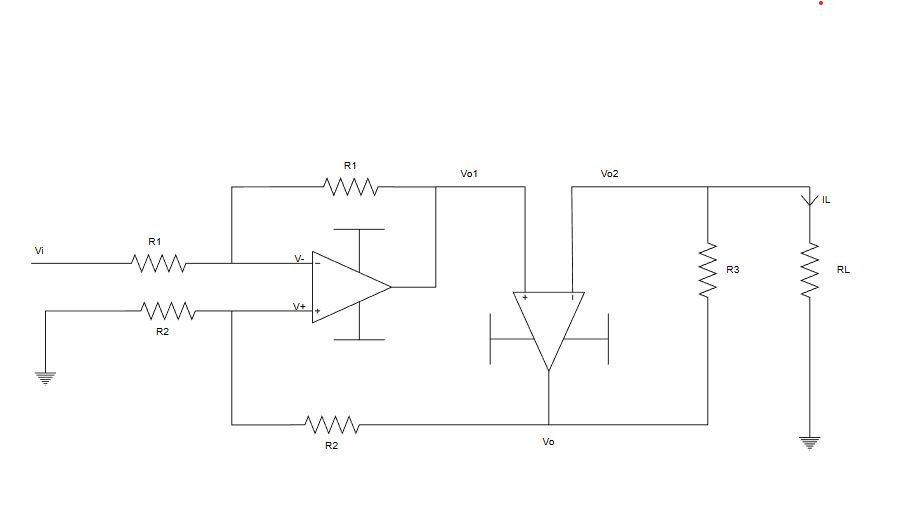
\includegraphics[width=.9\linewidth]{./my-chapters/my-images/Question2/câu 2 hình a.png}
\end{figure}

\begin{itemize}[label=-]
	\item OPAMP 1:
	\[ \dfrac{V_{o1} - V_{-}}{R_{1}} = \dfrac{V_{-} - V_{i}}{R_{1}} \Rightarrow V_{i} = 2V_{-} - V_{o1} \]
	\[ \Rightarrow V_{i} = 2V_{+} - V_{o1} \]
	\[ \dfrac{V_{o} - V_{+}}{R_{2}} = \dfrac{V_{+}}{R_{2}} \Rightarrow V_{o} = 2V_{+} \]
	\[ \Rightarrow V_{i} = V_{o} - V_{o1} \Rightarrow V_{o1} = V_{o} - V_{i} \]
	
	\item OPAMP 2:
	\[ V^{+} = V^{-} \Rightarrow \dfrac{V_{o} - V_{o2}}{R_{3}} = \dfrac{V_{o2}}{R_{L}} = I_{L} \]
	\[ \Rightarrow V_{o} = I_{L}R_{3} + V_{o2} \]
	Ta có:
	\[ V_{o1} = V_{o2} \Rightarrow V_{o} = I_{L}R_{3} + V_{o} - V_{i} \]
	\[ \Rightarrow V_{i} = I_{L}R_{3} \]
	
	$\Rightarrow$ \finalresult{I_{L} = \dfrac{V_{i}}{R_{3}}}
\end{itemize}

\answer{b1}{Giả sử cả 2 OPAMP ở hình 2a có $V_{io} = 100\,\mu\textsf{V}$, $I_{io} = 4\,\textsf{nA}$, $I_{ib} = 18\,\textsf{nA}$. Tìm ảnh hưởng của điều kiện không lý tưởng của OPAMP lên ngõ ra $I_{L}$.}

\begin{itemize}[label=-]
	\item Xét ảnh hưởng của $V_{io}$: Khi $V_{i} = 0$, $V_{io} \neq 0$, $I_{+} = I_{-} = 0$
	
	\begin{figure}[H]
		\centering
		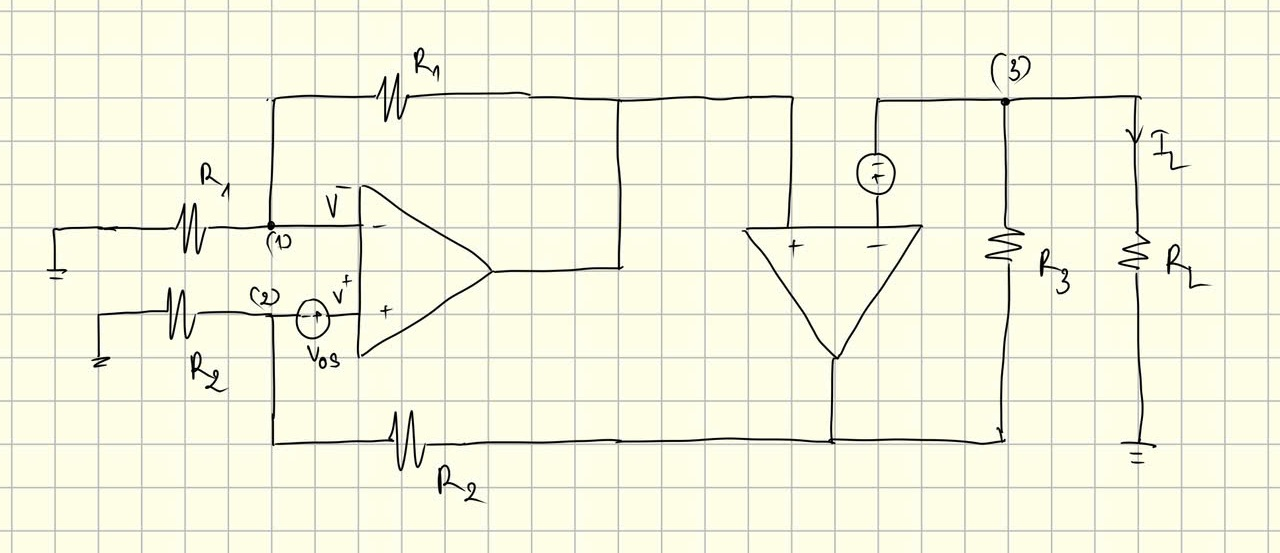
\includegraphics[width=.9\linewidth]{./my-chapters/my-images/Question2/câu 2 b hình a Vio.jpg}
		\caption{Ảnh hưởng của $V_{io}$ lên mạch 2a.}
	\end{figure}
	
	\begin{itemize}[label=+]
		\item Phương trình KCL tại nút (1):
		\[ \dfrac{V_{io}}{R_{1}} + \dfrac{V_{io} - V_{o1}}{R_{1}} = 0 \Rightarrow V_{o1} = 2V_{io} \]
		\item Phương trình KCL tại nút (2):
		\[ \dfrac{V_{io}}{R_{2}} + \dfrac{V_{io} - V_{o}}{R_{2}} = 0 \Rightarrow V_{o} = 2V_{io} \]
		\item Phương trình KCL tại nút (3):
		\[ \dfrac{V_{o1} - V_{io} - V_{o}}{R_{3}} + I_{L} = 0 \]
	\end{itemize}
	
	$\Rightarrow$ \finalresult{I_{L} = \dfrac{V_{io}}{R_{3}}}
	
	\item Xét ảnh hưởng của $I_{io},\ I_{ib}$: Khi $V_{i} = 0$, $V_{io} = 0$ và $I_{+} \neq I_{-} \neq 0$
	
	\begin{figure}[H]
		\centering
		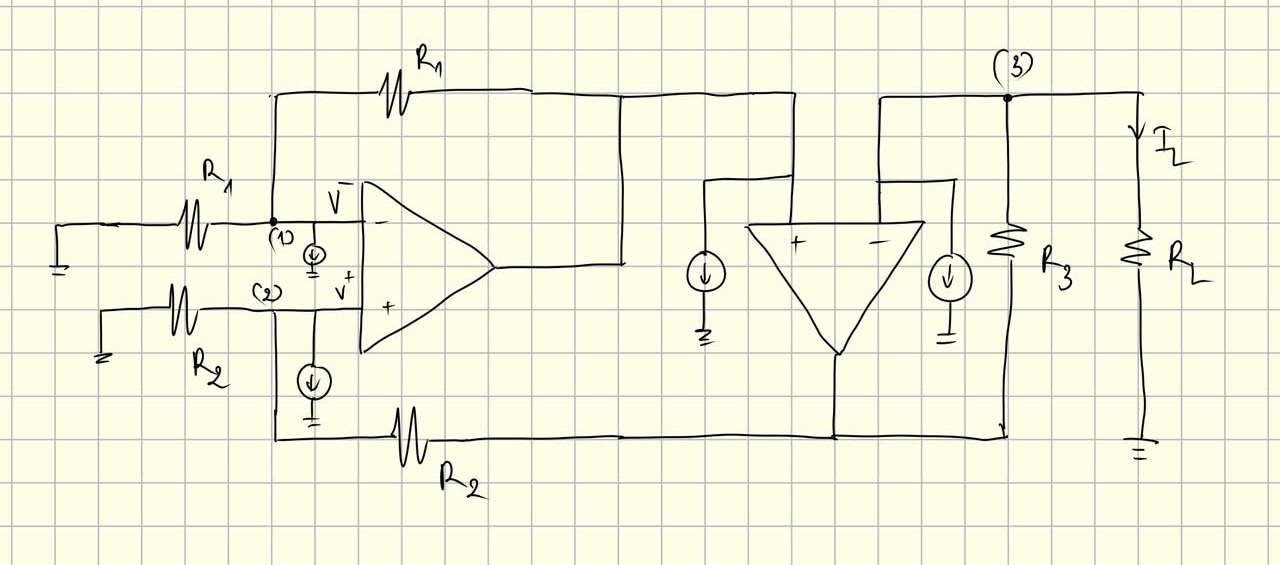
\includegraphics[width=.9\linewidth]{./my-chapters/my-images/Question2/Câu 2 b hình a Iio.jpg}
		\caption{Ảnh hưởng của $I_{io}$ và $I_{ib}$ lên mạch 2a.}
	\end{figure}
	
	\[
	\left\{
	\begin{matrix}
		| I_{+} - I_{-} | = I_{io} \\[4pt]
		I_{+} + I_{-} = 2I_{ib}
	\end{matrix}
	\right.
	\Rightarrow
	\left\{
	\begin{matrix}
		I_{+} = 16\,\text{nA} \\[4pt]
		I_{-} = 20\,\text{nA}
	\end{matrix}
	\right.
	\]
	
	\begin{itemize}[label=+]
		\item Phương trình KCL tại nút (1):
		\[ I_{-} + \dfrac{0 - V_{o1}}{R_{1}} = 0 \Rightarrow V_{o1} = I_{-}R_{1} \]
		\item Phương trình KCL tại nút (2):
		\[ I_{+} + \dfrac{0 - V_{o}}{R_{2}} = 0 \Rightarrow V_{o} = I_{+}R_{2} \]
		\item Phương trình KCL tại nút (3):
		\[ I_{-} + \dfrac{V_{o1} - V_{o}}{R_{3}} + I_{L} = 0 \]
	\end{itemize}
	
	$\Rightarrow$ \finalresult{I_{L} = -I_{-}\left(1 + \dfrac{R_{1}}{R_{3}}\right) + I_{+}\dfrac{R_{2}}{R_{3}}}
	
	\item Xét toàn mạch:
	
	Ảnh hưởng của $V_{io}$, $I_{io}$ và $I_{ib}$ lên mạch là:
	\finalresult{I_{L} =  \dfrac{V_{i}}{R_{3}} \pm \dfrac{V_{io}}{R_{3}} \pm \left( -I_{-}\left(1 + \dfrac{R_{1}}{R_{3}}\right) + I_{+}\dfrac{R_{2}}{R_{3}} \right) }
\end{itemize}

\answer{a2}{Giả sử OPAMP ở hình 2b đang dùng là lý tưởng.}

\begin{figure}[H]
	\centering
	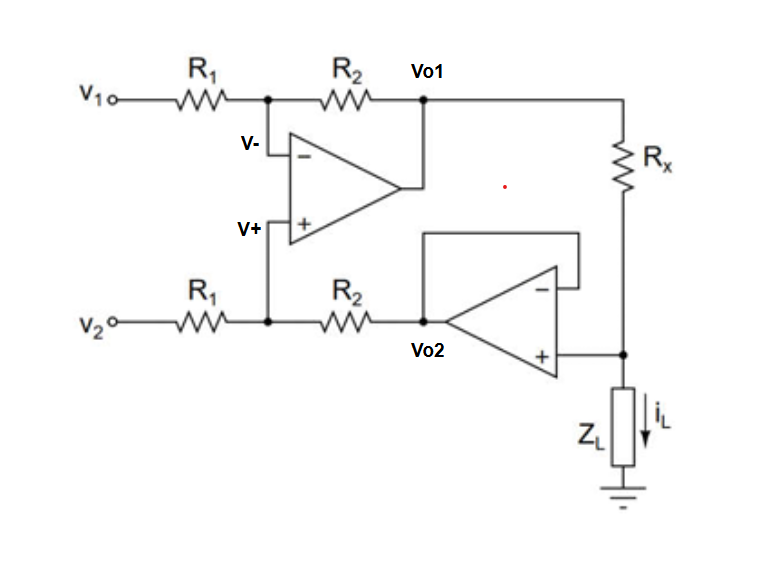
\includegraphics[width=.9\linewidth]{./my-chapters/my-images/Question2/Câu 2 hình b.png}
\end{figure}

\begin{itemize}[label=-]
	\item Opamp 1: Ta có: $V_{+} = V_{-}$
	
	\[ \dfrac{V_{o1} - V_{-}}{R_{2}} = \dfrac{V_{-} - V_{1}}{R_{1}} \Rightarrow V_{1} = \left(\dfrac{R_{1}}{R_{2}} + 1\right)V_{-} - \dfrac{R_{1}}{R_{2}}V_{o1} \]
	
	\item Opamp 2:
	
	\[ \dfrac{V_{o2} - V_{+}}{R_{2}} = \dfrac{V_{+} - V_{2}}{R_{1}} \Rightarrow V_{2} = \left(\dfrac{R_{1}}{R_{2}} + 1\right)V_{+} - \dfrac{R_{1}}{R_{2}}V_{o2} \]
	
	\item Ta có:
	
	\[ \dfrac{V_{o1} - V_{o2}}{R_{x}} = \dfrac{V_{o2}}{Z_{L}} = I_{L} \Rightarrow V_{o1} - V_{o2} = R_{x}I_{L} \]
	\[ V_{1} - V_{2} = -\dfrac{R_{1}}{R_{2}}\left(V_{o1} - V_{o2}\right) = -\dfrac{R_{1}}{R_{2}}R_{x}I_{L} \]
	
	$\Rightarrow$ \finalresult{I_{L} = -\dfrac{R_{2}}{R_{1}R_{x}}\left(V_{1} - V_{2}\right)}
\end{itemize}



\answer{b2}{Giả sử cả 2 OPAMP ở hình 2b có $V_{io} = 100\,\mu\textsf{V}$, $I_{io} = 4\,\textsf{nA}$, $I_{ib} = 18\,\textsf{nA}$. Tìm ảnh hưởng của điều kiện không lý tưởng của OPAMP lên ngõ ra $I_{L}$.}

\begin{itemize}[label=-]
	\item Xét ảnh hưởng của $V_{io}$: Khi $V_{1} = V_{2} = 0$, $V_{io} \neq 0$ và $I_{+} = I_{-} = 0$
	
	\begin{figure}[H]
		\centering
		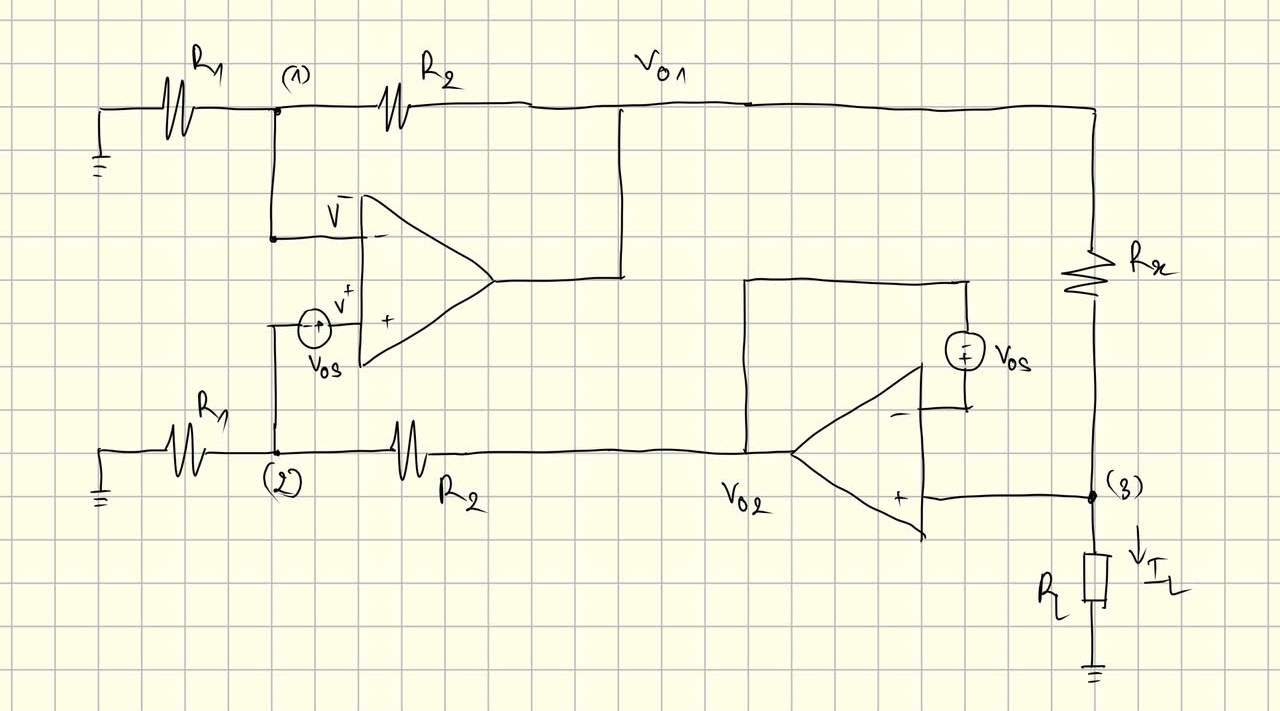
\includegraphics[width=.9\linewidth]{./my-chapters/my-images/Question2/câu 2 b hình b Vio.jpg}
		\caption{Ảnh hưởng của $V_{io}$ lên mạch 2b.}
	\end{figure}
	
	\begin{itemize}[label=+]
		\item Phương trình KCL tại nút (1):
		\[ \dfrac{V_{io}}{R_{1}} + \dfrac{V_{io} - V_{o1}}{R_{2}} = 0 \Rightarrow V_{o1} = \left(1 + \dfrac{R_{2}}{R_{1}}\right)V_{io} \]
		\item Phương trình KCL tại nút (2):
		\[ \dfrac{V_{io}}{R_{1}} + \dfrac{V_{io} - V_{o2}}{R_{2}} = 0 \Rightarrow V_{o2} = \left(1 + \dfrac{R_{2}}{R_{1}}\right)V_{io} \]
		\item Phương trình KCL tại nút (3):
		\[ \dfrac{V_{io} - V_{o2} - V_{o1}}{R_{x}} + I_{L} = 0 \]
		\[ \Rightarrow I_{L} = \dfrac{-V_{io} + \left(1 + \dfrac{R_{2}}{R_{1}}\right)V_{io} + \left(1 + \dfrac{R_{2}}{R_{1}}\right)V_{io}}{R_{x}} \]
	\end{itemize}
	
	$\Rightarrow$ \finalresult{I_{L} = \dfrac{\left(1 + \dfrac{2R_{2}}{R_{1}}\right)V_{io}}{R_{x}} = \dfrac{R_{1} + 2R_{2}}{R_{x}R_{1}}{V}_{io}}
	\\
	\begin{figure}[H]
		\centering
		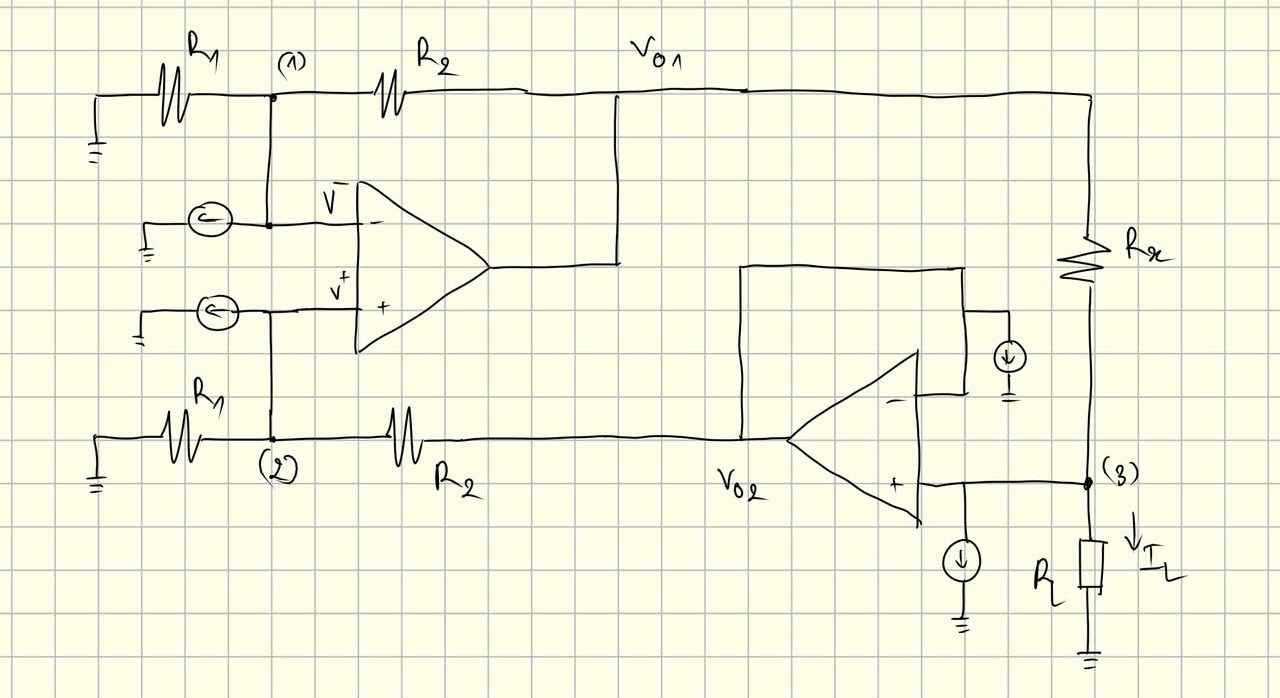
\includegraphics[width=.9\linewidth]{./my-chapters/my-images/Question2/câu 2 b hình b Iio.jpg}
		\caption{Ảnh hưởng của $I_{io}$ và $I_{ib}$ lên mạch 2b.}
	\end{figure}
	
	\item Xét ảnh hưởng của $I_{io},\ I_{ib}$: Khi $V_{1} = V_{2} = 0$, $V_{io} = 0$ và $I_{+} \neq I_{-} \neq 0$
	
	\[
	\left\{
	\begin{matrix}
		| I_{+} - I_{-} | = I_{io} \\[4pt]
		I_{+} + I_{-} = 2I_{ib}
	\end{matrix}
	\right.
	\Rightarrow
	\left\{
	\begin{matrix}
		I_{+} = 16\,\text{nA} \\[4pt]
		I_{-} = 20\,\text{nA}
	\end{matrix}
	\right.
	\]

	\begin{itemize}[label=+]
		\item Phương trình KCL tại nút (1):
		\[ I_{+} + \dfrac{0 - V_{o}}{R_{2}} = 0 \Rightarrow V_{o} = I_{+}R_{2} \]
		\item Phương trình KCL tại nút (2):
		\[ I_{-} + \dfrac{0 - V_{o1}}{R_{1}} = 0 \Rightarrow V_{o1} = I_{-}R_{1} \]
		\item Phương trình KCL tại nút (3):
		\[ I_{-} + \dfrac{V_{o1} - V_{o}}{R_{3}} + I_{L} = 0 \]
	\end{itemize}
	
	$\Rightarrow$ \finalresult{I_{L} = -I_{-}\left(1 + \dfrac{R_{1}}{R_{3}}\right) + I_{+}\dfrac{R_{2}}{R_{3}}}
	
	\item Xét toàn mạch:
	
	Ảnh hưởng của $V_{io}$, $I_{io}$ và $I_{ib}$ lên mạch là:\\
	\finalresult{I_{L} = -\dfrac{R_{2}}{R_{1}R_{x}}\left(V_{1} - V_{2}\right) \pm \left( \dfrac{R_{1} + 2R_{2}}{R_{x}R_{1}}{V}_{io} \right) \pm \left( -I_{-}\left(1 + \dfrac{R_{1}}{R_{3}}\right) + I_{+}\dfrac{R_{2}}{R_{3}} \right) }
\end{itemize}
